%%==================================================
%% chapter04.tex for BIT Master Thesis
%% modified by yang yating
%% version: 0.1
%% last update: Dec 25th, 2016
%%==================================================
\chapter{ReL4系统实现}
\label{chap:ReL4_impl}

为了简洁高效地实现异步微内核的原型系统,本项目使用Rust语言在RISC-V平台上实现了一个兼容seL4的微内核ReL4,目前已经支持SMP架构和fast-path优化。在兼容seL4原始功能的基础(包括SMP和fast-path优化)上, ReL4实现了U-notification以及异步IPC和异步系统调用。在实现过程中对内核接口更改和使用的一些重要细节将在本章描述。

\section{新增系统调用}

\begin{table}
    \centering
    \begin{tabular}{|c|c|c|}
        \hline 
        syscall & 参数 & 描述 \\
        \hline
        UintrRegisterSender & ntfn\_cap & 注册通知发送端 \ \\
        \hline
        UintrRegisterReceiver & ntfn\_cap & 注册通知接收端 \ \\
        \hline
        UintrRegisterAsyncSyscall & ntfn\_cap, buffer\_cap & 注册异步系统调用处理协程 \ \\
        \hline
        UintrWakeSyscallHandler & - & 唤醒系统调用处理协程 \ \\
        \hline
    \end{tabular}
    \caption{ReL4中的新增系统调用}
    \label{tab:new_syscall}
\end{table}

如\ref{tab:new_syscall}所示,为了支持内核对U-notification的硬件资源管理,ReL4新增了系统调用:UintrRegisterSender 和 UintrRegisterReceiver 用于申请相关的硬件资源,其参数是notification内核对象对应的Capbability。内核会从UINTC中分配对应的硬件寄存器索引,并将对应的索引绑定到TCB中,资源的释放不需要额外的系统调用,当TCB或notification对象销毁时会自动释放掉硬件资源。

此外,为了支持异步系统调用,共享缓冲区也需要通过系统调用(UintrRegisterAsyncSyscall)注册给内核,内核会为将共享缓冲区与TCB绑定,并为该线程注册处理该缓冲区请求的内核协程。最后,由于用户态中断不支持用户态直接通知内核态,内核提供一个用于唤醒系统调用处理协程的系统调用UintrWakeSyscallHandler,内核会将对应的处理协程唤醒,并找到一个空闲的CPU核心发送核间中断去抢占执行。

为了对seL4进行兼容,这些系统调用均由异步运行时在初始化时进行调用,用户程序无需感知。

\section{异步IPC}

异步IPC作为ReL4中的主要的IPC方式,其实现依赖于异步运行时和U-notification。以IPC中最常见的Call为例,如\ref{fig:async_ipc}所示,客户端进程和服务端进程在双方建立连接时,首先会想内核申请两条通道所占用的硬件资源,然后每个进程中的runtime会注册一个dispatcher协程并将绑定0号中断向量,用于在TAIC资源不够的情况下,用软件方式唤醒worker协程。服务端和客户端的worker协程则负责发起和处理请求,由runtime将数据写入共享缓冲区中。由于中断向量有限,runtime会尝试为每个worker协程分配中断向量,分配到中断向量的协程,其唤醒过程由TAIC完成,没有分配到中断向量的协程,其唤醒过程由dispatcher协程完成。

\begin{figure*}[htbp]
    \centering
    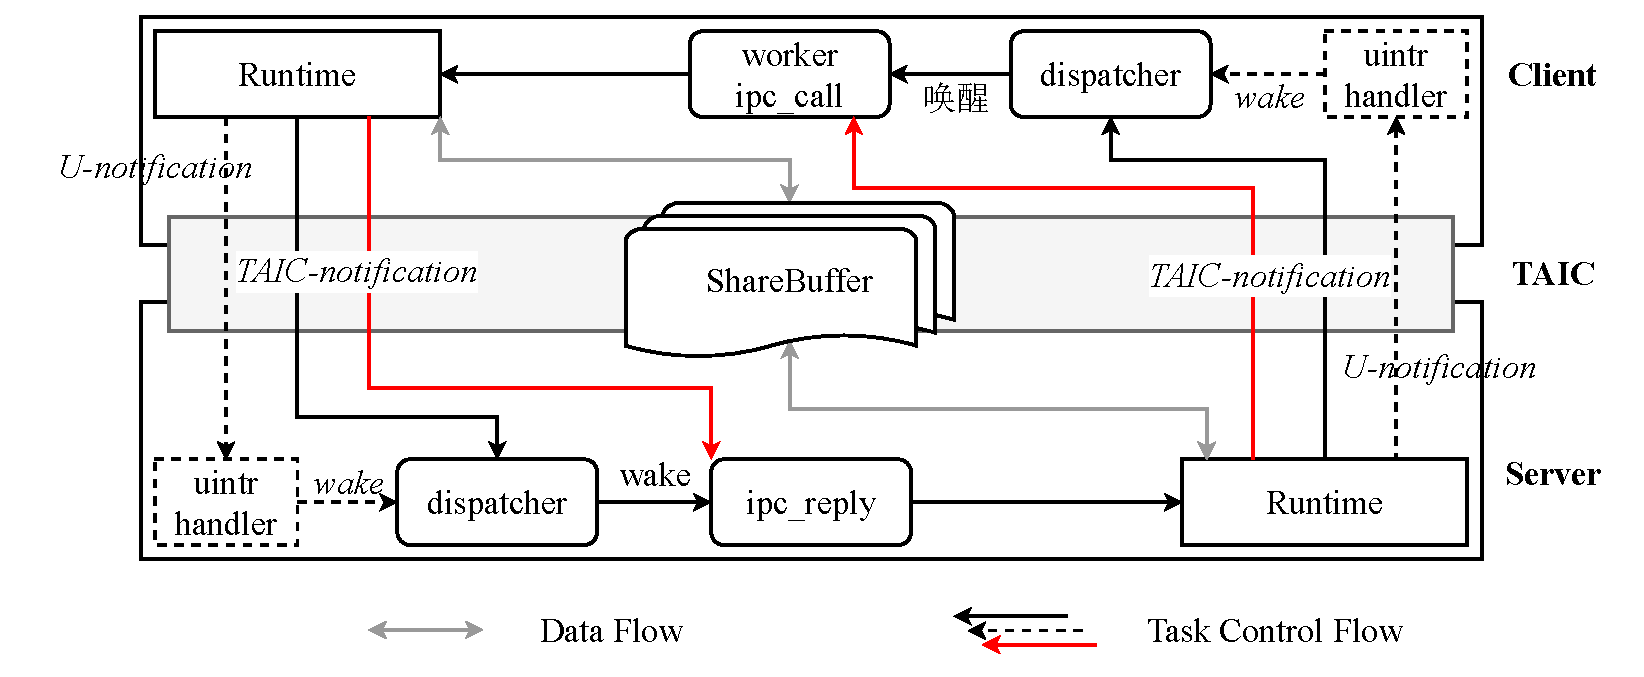
\includegraphics[width=0.9\textwidth]{figures/async_ipc.drawio.pdf}
    \caption{调度器的结构图}\label{fig:async_ipc}
  \end{figure*}

Call的主要流程分为以下几个阶段:
\begin{enumerate}
    \item 客户端发起请求:用户态程序将以worker协程的形式发起IPC请求,异步运行时首先会尝试分配一个中断向量给worker协程,如果如果没有分配到,则复用dispatcher协程的0号中断,然后根据请求的数据和协程的协程号、中断号生成 IPCItem 并写入请求的环形缓冲区中并将当前协程阻塞,然后检查缓冲区的 $req\_handler\_status$ 标志位,如果对方的dispatcher协程已经就绪,那客户端无需通知对方进程,对方进程的异步运行时会在某个时刻调度到dispatcher协程并处理请求。如果对方的dispatcher协程处于阻塞状态,则异步运行时会将$req\_handler\_status$ 标志位置位,并发送U-notification通知对方进程唤醒 dispatcher协程并重启调度。
    \item 服务端处理请求并写回响应:服务端的dispatcher协程会在合适的时机读取出请求并进行解码和处理,然后根据处理结果构造响应的 IPCItem 并写入响应的环形缓冲区中,如果中断号是0号协程,则runtime会检查缓冲区中的 $req\_handler\_status$  标志位后尝试唤醒客户端的 dispatcher协程,否则直接通过TAIC唤醒客户端的worker协程。如果缓冲区内容为空,dispatcher协程会将 $req\_handler\_status$  标志位置空,并将自己阻塞。
    \item 客户端处理响应:客户端的 dispatcher协程会在合适的时机重新被调度并唤醒没有分配到TAIC资源的worker协程,唤醒后的worker协程会从缓冲区中读取响应并释放缓冲区资源。
\end{enumerate}

其伪代码如\ref{alg:async_ipc}所示。

\begin{algorithm}[H]
    \caption{异步IPC流程的伪代码}\label{alg:async_ipc}
    \SetKwFunction{Fn}{fn}
    \SetKwProg{Prog}{}{}{}
    \SetKw{KwAwait}{await}
    \SetKw{KwYield}{yield\_now}
    \SetKw{KwLet}{let}
    \SetKw{KwSome}{Some}
    \SetKw{KwErr}{Err}
    \SetKw{KwReturn}{return}
    
    \Prog{\Fn{async ipc\_call(cap, msg\_info) $\rightarrow$ Result<IPCItem>}}{
        vec = get\_vec\_from\_pool()\;
        item = IPCItem::new(vec, current\_cid(), msg\_info)\;
        buffer = get\_buffer\_from\_cap(cap)\;
        buffer.req\_ring\_buffer.write(item)\;
        \If{buffer.req\_co\_status == false}{
            buffer.req\_co\_status = true\;
            u\_notification\_signal(0)\;
        }
        \If{\KwLet \KwSome(reply) = \KwYield().\KwAwait}{
            \KwReturn \KwSome(reply)\;
        }
        \KwReturn \KwErr(())\;
    }
    
    \Prog{\Fn{async ipc\_recv\_reply(cap)}}{
        buffer = get\_buffer\_from\_cap(cap)\;
        \While{true}{
            \If{\KwLet \KwSome(item) = buffer.req\_ring\_buffer.get()}{
                reply = handle\_item(item)\;
                buffer.resp\_ring\_buffer.write(reply)\;
                \If{buffer.reply\_co\_status == false}{
                    buffer.reply\_co\_status = true\;
                    u\_notification\_signal(item.vec)\;
                }
            }\Else{
                buffer.req\_co\_status = false\;
                \KwYield().\KwAwait\;
            }
        }
    }
\end{algorithm}



\section{异步系统调用}
从广义的角度来看,异步系统调用是一类特殊的异步IPC,其接收方为内核。因此ReL4在内核中提供了一套相似的异步运行时以支持异步系统调用。异步系统调用与异步IPC的主要不同之处有两点:
\begin{enumerate}
    \item 由于接收端是内核,发送端无法使用U-notification去通知内核。
    \item 异步IPC中进程的异步调度器就是进程的执行主体,无需考虑异步任务的执行时机,而内核除了异步系统调用请求需要调度器执行,本身就有如中断、异常、任务调度等其他任务需要被执行。
\end{enumerate}

对于第一点,ReL4新增一个系统调用去用于唤醒相关的内核协程即可。而对于第二点,一个很简单的思路是每次时钟中断到来时去执行异步系统调用,然而这可能会导致空闲的CPU核心无法及时触发时钟中断而空转,因此,在不破坏原本的线程优先级调度前提下,ReL4使用核间中断来抢占空闲CPU核心或正在运行低优先级线程的CPU核心,更好地利用空闲CPU资源,减少响应时延。

为了避免破坏微内核中原本的优先级调度机制,ReL4在内核中对每个CPU核心维护了相应的执行优先级($exec\_prio$),执行优先级区别于上文提到的运行时协程优先级,是由内核调度器维护的线程优先级。内核中的任务主要分为三类:
\begin{enumerate}
  \item idle thread: 空闲CPU核心执行idle线程,此时CPU核心的执行优先级为256,属于最低的执行优先级。
  \item 内核态任务:正在处理中断、异常、系统调用等,此时CPU核心的执行优先级为0,最高优先级,不可被抢占。
  \item 用户态任务:正在执行用户态的任务,此时CPU核心的执行优先级为当前线程的优先级,可以被更高优先级线程提交的异步系统调用请求打断。
\end{enumerate}


当发送端通过系统调用陷入内核去唤醒相应协程后,会检查当前线程的优先级是否可以抢占其他CPU核心,如果可以,则发送核间中断抢占该CPU核心去执行异步系统调用,当前CPU核心则返回用户态继续执行其他协程。如果没有可以被抢占的CPU核心,则在下一次时钟中断到来时执行异步系统调用请求,其伪代码\ref{alg:wake_syscall_handler}所示:

\lstdefinelanguage{rust}{
    keywords={fn, if, let, Some, as, in},
    keywordstyle=\color{blue}\bfseries,
    ndkeywords={self, current, cid, cpu_id, exec_prio, mask},
    ndkeywordstyle=\color{magenta}\bfseries,
    identifierstyle=\color{black},
    sensitive=false,
    comment=[l]{//},
    morecomment=[s]{/*}{*/},
    commentstyle=\color{gray}\ttfamily,
    stringstyle=\color{red}\ttfamily,
    morestring=[b]',
    morestring=[b]"
}

\begin{algorithm}[H]
    \caption{唤醒内核中异步处理协程的伪代码}\label{alg:wake_syscall_handler}
    \SetKwFunction{Fn}{fn}
    \SetKwProg{Prog}{}{}{}
    \Prog{\Fn{wake\_syscall\_handler()}}{
        current = get\_current\_thread(); \\
        \If{let Some(cid) = current.async\_sys\_handler\_cid} {
            coroutine\_wake(cid); \\
            current\_exec\_prio = current.tcb\_prio; \\
            (cpu\_id, exec\_prio) = get\_max\_exec\_prio(); \\
            \If{current\_exec\_prio < exec\_prio} {
                // 抢占低执行优先级的核心 \\
                mask = 1 $\ll$ cpu\_id; \\
                ipi\_send\_mask(mask, ASYNC\_SYSCALL\_HANDLE); \\
            }
        }
    }
\end{algorithm}

\section{兼容性讨论}
\label{sec:rel4_comp}
为了提升用户态程序的易用性,ReL4对seL4的程序提供一定的兼容性。ReL4中已经实现了seL4的基本系统调用并支持对称多处理机(SMP),但采用不同的通知机制和IPC设计和系统调用处理机制,因此有必要讨论这两部分的兼容性。

\subsection{Notification与U-notification}

相比于原始的通知机制,U-notification在通信权限控制方面同主要存在以下两点不同:

\begin{enumerate}
  \item 原始的通知机制允许多个接收线程竞争接收一个内核对象上的通知,这种设计的目的是为了支持多接收端的场景,事实上,多接收端已经通过多个内核对象来进行支持,因此这种机制相对冗余,而由于U-notification中接收端对接收线程的独占性,这个能力将不再被支持。
  \item 原始的通知机制允许单个接收线程接收多个内核对象上的通知,这种设计的目的是更灵活地支持多发送端的场景,在U-notification中,同一个内核对象可以被设置为相同的recv status idx,不同的发送端则通过使用中断号(uintr vec)来进行区分。
\end{enumerate}

除了权限控制有所不同之外,改造前后的通信方式也有所区别。原始的通知机制需要用户态接收方通过系统调用主动询问内核是否有通知需要处理。根据是否要将线程阻塞,一般被设计为Wait和Poll两个接口。而U-notification无需接收线程主动陷入并询问内核,接收方被硬件发起的用户态中断打断,并处理到来的通知,这在很大程度上解放了接收方,程序设计者无需关心通知到来的时机,减少了CPU忙等的几率,提升了用户态的并发度。而为了提升U-notification的易用性,ReL4对原始的通信接口进行了兼容:
\begin{enumerate}
  \item Poll: 无需陷入内核态,在用户态读取中断状态寄存器,判断是否有效并返回。
  \item Wait: 对该接口的兼容需要用户态的异步运行时的调度器提供相关支持	,在没有有效中断时,该操作将阻塞当前协程并切换到其他协程执行,等待用户态中断唤醒。
\end{enumerate}

综上所述,对于多接收方的场景,U-notification可以通过多个内核对象进行实现,除此之外,U-notification可以实现API级别的兼容。

\subsection{同步IPC与异步IPC}

异步IPC通过异步运行时可以在基本通信场景下上实现API级别的兼容,然而seL4中的同步IPC还有额外的能力:
\begin{enumerate}
  \item 	错误处理:同步IPC可以用于缺页异常等处理,seL4通过在TCB中维护一个Endpoint对象来发送错误信息给用户态程序进行处理,而在ReL4中,TCB中将维护对应的U-notification对象,以及对应的共享缓冲区指针,当异常和错误发生时,将错误信息写入共享缓冲区,并发送U-notification通知用户态程序。此场景下依然可以实现API级别的兼容。
  \item 能力派生:seL4中的同步IPC拥有能力派生与传递的功能,虽然内核已经支持了Capability Space相关的系统调用,同步IPC使得能力传递更加灵活。而由于异步IPC不经过内核,因此ReL4中不再支持通过IPC来进行能力派生,仅通过系统调用进行能力派生,损失了一部分灵活性,保留了功能的完整性。
\end{enumerate}

此外,异步运行时导致用户态任务模型存在语义上的区别,异步IPC任务将以协程作为任务的基本单位,因此相比于同步IPC任务之外,异步IPC提供了主动让权的API,同时,相比于同步IPC,相同运行时内的不同异步IPC任务不存在并行性,无需同步互斥等操作,提升了用户态易用性。

综上所述,异步IPC在大部分情况下依然能实现API级别的兼容。

\subsection{同步系统调用于异步系统调用}
与异步IPC类似,异步系统调用的发起依然以协程为单位进行,但与同步系统调用的处理不同,为了充分利用CPU硬件,异步系统调用的处理采用多核心、抢占式处理,如果系统中存在空闲核心或执行低优先级任务的核心,异步系统调用会抢占该核心并处理系统调用请求,因此系统调用的发起和处理有可能是多核心且并行的。

此外,有两类系统调用无法异步化:
\begin{enumerate}
  \item 由于异步系统调用依赖于异步运行时,因此与异步运行时初始化相关的系统调用无法被异步化。
  \item 对于实时性要求较高的系统调用无法进行异步化,如$get\_clock()$。
\end{enumerate}

对于上述两类,我们通过异步运行时中的API兼容层进行自动判断,对于无法异步化的系统调用,运行时将自动转化为同步系统调用进行处理。综上所述,异步系统调用可以实现API级别的兼容。

